% !TEX root = ../main.tex

\chapter{Scope}\label{chap:scope}

This chapter is devoted to a brief overview of the state-of-the-art in \ac{TTS} technology and it will serve as a way of contextualizing the scope of my work within the field.

In the first section of the chapter, I will centre the discussion around the dominant \ac{TTS} paradigms and the role that \ac{F0} modeling plays within them.
This serves as justification for the \ac{TTS} paradigm that was selected for the implementation of the proposed methodology.

The second section will be devoted to the discussion of models of intonation.
In this section, I will offer a brief review of some of the historically most influential models of intonation.

In the third section, I will outline a deep learning methodology for the modeling of intonation.
The methodology is contextualized and compared with previous research.


\section{TTS Paradigms}\label{sec:tts-paradigms}

\ac{TTS} technology can be divided into two main branches.
On the one hand, we have rule-based synthesis and on the other we have corpus-based synthesis.

In rule-based synthesis, which is historically highly related to formant-synthesis, expert knowledge is required to come up with rules that adequately account for speech phenomena.
This knowledge is expensive to acquire, it does not apply cross-linguistically, and it does not produce very natural sounding speech, as it is almost impossible for experts to describe any meaningful size of the combinatory space by means of rules.

Most rule-based intonation systems are inspired by the Pierrehumbert model and make use of some variation of  the \ac{ToBI} transcription system \citep{Silverman1992ToBI}.

The main advantage of rule-based approaches is that it can be very flexible and it can have a very small footprint.
Even though this technology has largely been surpassed by corpus-based synthesis, rule-based synthesis is still been used for some limited applications, where footprint might be a concern or when no speech data is available.


The second major approach to \ac{TTS} is corpus-based synthesis.
Within this approach, we do not try to come up with linguistic rules that describe speech phenomena, but rather we try to build models or databases from speech corpora.

As this approach is currently regarded as the state-of-the-art, the following sections will be devoted to two main paradigms of corpus-based synthesis: \ac{USS} and \ac{SPSS}.

\subsection{Unit Selection Synthesis}

\ac{USS} is based on the use of original speech signals found in speech corpora, where units of speech are dynamically selected from the corpus at run-time.
The selection process, in this case, is guided by the concerted effort of minimizing target costs (i.e., how close the candidate is to our target specification) and concatenative costs (i.e., how well the candidate fits with adjacent units).

Many of the foundational ideas behind this approach were first laid out in \citet
{Hunt1996Unit} and \citet{Campbell1997Prosody}, which quickly lead to the development of systems based on this new approach.
The success of this approach is due to the fact that, despite its simplicity, it can produce highly intelligible and highly natural synthetic speech.

However, \ac{USS} is not very flexible with regard to intonation modeling.
This is because most \ac{USS} systems adopt a so-called ``as-is'' approach, whereby the problem of prosody is tackled only indirectly by including prosodic information in the target and concatenative cost functions.
This is under the assumption and the hope that the system will happen to find appropriate segments that also fit together.

However, because of the extremely high levels of sparsity that characterize most language and speech phenomena \citep{Santen1997Combinatorial, Moebius2003Rare}, \ac{USS} approaches will often lead to noticeable prosodic discontinuities when no appropriate units can be found.
This problem is alleviated in most \ac{USS} systems by designing the corpus to include fairly neutral news-style speech, which can be problematic if one wishes to generate expressive and affective speech.

These issues relating to \ac{F0} modeling constraints can be better illustrated by the example in \autoref{tab:uss-corpus}, where we can imagine how a unit selection system would operate in order to predict the \ac{F0} contour of the target sentence, provided that sentences 1, 2, 3, and 4 are our entire corpus. 

The system would completely ignore sentence 1 and splice together the boldface segments from sentence 2, 3, and 4. 
This is due to the fact that the target sentence and sentence 1 have very little in common as far as phone sequence is concerned.

\begin{table}[h!]
\begin{center}
\begin{tabular}[c]{| c | c |}
\hline
\textbf{Target} & Earlier, I drank a small glass of fizzy coke.\\
\hline
                & (1) Clearly, she has a real knack for funny jokes.\\
\textbf{Corpus} & (2) \textbf{I} met your husband \textbf{earlier}.\\
                & (3) Did you say she \textbf{drank a small glass} of water?\\
                & (4) A nice bottle \textbf{of fizzy coke} is what is needed \\
                &   on a hot summer day!\\
\hline
\end{tabular}
\end{center}
\caption[Unit selection speech corpus.]{Example of a speech corpus, where the second row contains the speech corpus used by a  system for the synthesis of the target utterance contained in the first row.}
\label{tab:uss-corpus}
\end{table}

As we can see, intonation of the boldface segments would not match what is required for the target sentence. 

For instance, ``earlier'' in sentence 2 would have a far flatter and descending \ac{F0} compared to the target, because that is what we expect at the end of a declarative sentence. 
The segment ``drank a small glass'' comes from a question and the \ac{F0} will be rising too much for our needs. 
Finally, ``of fizzy coke'' is probably going to have a really upbeat and lively intonation because it's contained in an exclamatory utterance. 

However, we can easily make an argument that the intonation from sentence 1 would be a far more suitable candidate that the intonation generated from the combination of the boldface segments.
Unfortunately, \ac{USS} systems are unable to make use of prosodically more appropriate segments as these will rarely satisfy the phone-driven target specification.
This entails that even though the corpus might be rich in useful prosodic information, it will remain largely unused.



\subsection{Statistical Parametric Speech Synthesis}


After almost over a decade dominated by \ac{USS}, where the task of speech synthesis was essentially reduced to a highly sophisticated talking clock, we have recently been witnessing to a resurgence of older approaches, but revisited in the light of new ideas and technology.
One such example is \ac{SPSS}.

In \ac{SPSS}, we do not concatenate or manipulate the original pre-recorded waveforms, but rather, signals are synthesized from scratch, similarly to what used to be done in formant synthesis.

The main innovation of \ac{SPSS} lies in reframing the problem as a \ac{ML} task.
Unlike formant synthesis, we no longer try to come up with expert-knowledge rules, but we use \ac{ML} algorithms to automatically infer statistical models that describe mappings between sets of input features and output features.

The main difference with \ac{USS} is that, in \ac{SPSS}, we do not use data directly in the output, as we only use the corpus to extract linguistic and acoustic features that can later be used to train models.
In \ac{USS}, we can never do away with the original data, whereas in \ac{SPSS}, once we train a model, we no longer need the original waveforms to synthesize new utterances.
In \ac{USS}, we do not have a model proper, but something more akin to a database, as none of the original data has been parametrized.

The reason why research on alternatives to \ac{USS} such as \ac{SPSS} and articulatory synthesis is so active is because of the flexibility these alternative approaches can offer.
Unlike \ac{USS}, where our control is limited to how snippets of the pre-recorded waveform can be arranged, in parametric approaches, we theoretically have absolute control over every aspect of speech production, including duration, pitch, spectral features, etc.
This freedom comes from the fact that we are no longer dealing with cumbersome data that we cannot easily manipulate without significant signal degradation.
As signals are synthesized from scratch, we can define and set the parameters that are necessary to generate the speech phenomena that we want to capture.

This is especially important with regard to the \ac{F0}, an aspect that has been particularly hard to control under the unit selection paradigm, with the consequence that intonation modeling for a long time was mostly subordinated to the modeling of segmental features.
In \ac{SPSS}, it is possible to build models of intonation independently of other aspects of speech.
This means we have far more freedom to experiment with different approaches without worrying too much about other aspects of speech production. 

Although the classical way of describing \ac{TTS} systems is in terms of front-end and back-end, my overview will be structured in terms of an online and offline stage.
As the front-end is usually quite similar for most \ac{TTS} systems, it is more useful to structure the overview in terms of a more general \ac{ML} approach, where we often distinguish between an offline stage (i.e., training) and an online stage (i.e., inference).
\autoref{fig:spss-pipeline} shows the pipeline of a typical \ac{SPSS} system.
 
\vfill
\begin{figure}[h]
    \centering
    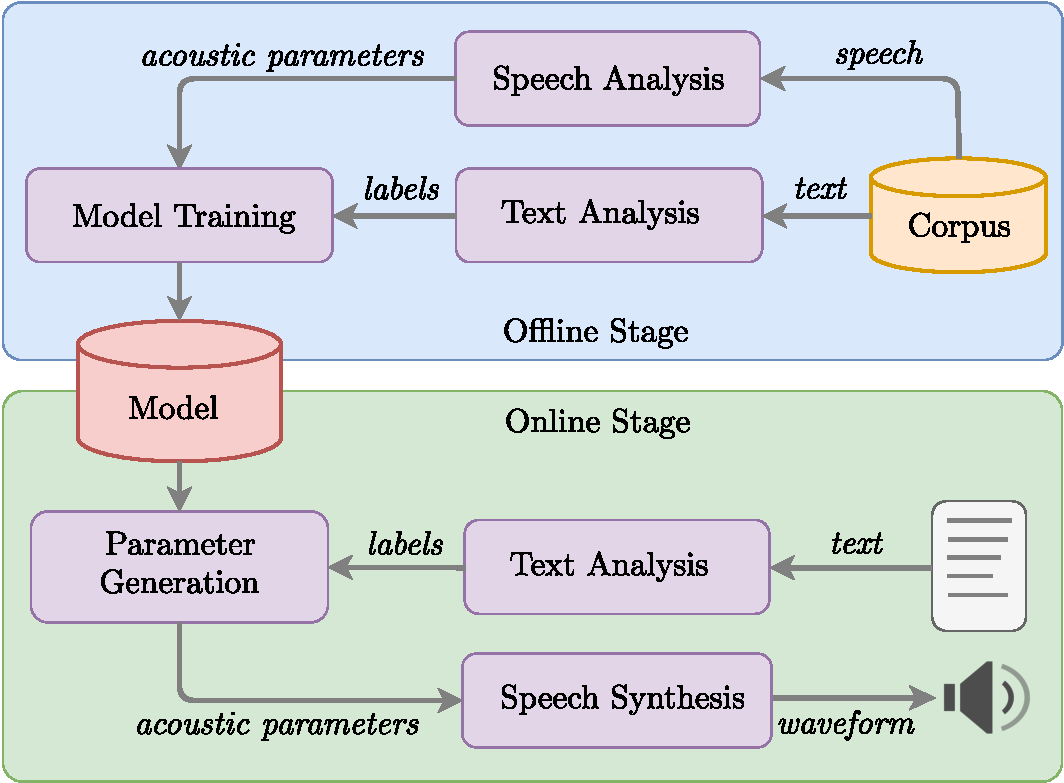
\includegraphics[scale=0.7]{figures/spss-pipeline.pdf}
    \caption[SPSS pipeline]{Pipeline of a typical \ac{SPSS} system. The blue box represents the offline stage, whereas the green one the online one.}
    \label{fig:spss-pipeline}
\end{figure}


\subsubsection{The Offline Stage}

In the offline stage (the blue box in \autoref{fig:spss-pipeline}), we first compile a speech corpus, i.e., a collection of audio material and its corresponding text, which is going to function as the training data.

From the corpus, we extract speech and textual features.
The input and output features must be aligned along the time domain.
This can be achieved by means of manual corpus annotation, or by means of forced alignment.

A text analysis component extracts labels that are used to construct a linguistic specification.
The linguistic specification usually contains information about phone labels, stress, \ac{POS} tags, etc.

A speech analysis components extracts output features in the form of acoustic parameters that can be used by a wave synthesizer to generate a waveform.
The exact nature of the acoustic parameters will largely depend on the selected wave synthesis mechanism.

The most common approach is to utilize a vocoder, which can decompose waveforms into acoustic parameters.
Many commonly used vocoders are based on the source-filter theory of speech, which arose from the merging of various theories on speech and acoustics \citep{Chiba1941vowel, Fant1960Acoustic}.
Two very commonly used vocoders are STRAIGHT \citep{Kawahara1999Restructuring} and WORLD \citep{Morise2016WORLD}.
These vocoders can produce reasonably intelligible speech, but they are also infamously known for the buzzing quality of the synthetic signal.

There exists a different class of vocoders, which completely ignore the source-filter model of speech and instead are based on sinusoidal modeling mechanisms \citep{McAulay1986Speech}.
An open-source example of these vocoders proposed recently is the MagPhase vocoder \citep{Espic2017Direct}.
These vocoders produce much better speech quality, but they are harder to use in real-world speech applications.

The labels produced by the text analysis component and the acoustic parameters extracted by the speech analysis component are then used to train a model that learns mappings from input to output features.
\acp{HMM} and \acp{DNN} are the two most common approaches for the training of the model.

The first \ac{SPSS} systems were based on \ac{HMM} approaches.
Even though they are quite effective, they are also plagued by a number of limitations.
As pointed out in \citet{Zen2013Statistical}, decision trees and \acp{GMM}, which are a big part of \ac{HMM} approaches, are not particularly suited for the modeling of complex long-term dependencies, causing the speech to be less varied and fairly monotonous.
Decision trees are also not particularly suited to approximating complex functions, at least not without building prohibitively large models.
Finally, decision trees tend to partition the input space into smaller regions, which results in a very fragmented representation of the input space.
This is very inefficient, as it requires the use of separate sets of parameters for each region.
It has been shown that this can lead decision trees to completely ignore weak or rare input signals, such as word-emphasis \citep{Yu2010Word}.

All of these issues, coupled with the recent emergence of deep-learning technology, have propelled the almost exclusive adoption of neural networks in almost every domain of speech technology.
Most neural networks used nowadays in deep learning are sets of algorithms based on mathematical models loosely inspired by biological neurons.
The power of neural networks rests on their ability to function as universal approximators, which endows them with the capacity to recognize and model extremely complex patterns.

\acp{DNN} solve many of the shortcomings affecting \ac{HMM}-based systems.
\acp{DNN} can model very complicated functions, they can make use of weak or rare input signals, they can deal with very high-dimensional and highly correlated features and they produce very compact and distributed representations, which means model parameters are used much more efficiently.
These properties are all highly desirable when solving very complicated problems such as speech and language tasks, where it is not at all uncommon to have to deal with very sparse and high-dimensional input spaces and where features interact in a very subtle and hierarchically layered fashion.

Over the last few years, a large body of research has emerged in which researchers have attempted to make use of \acp{DNN} to model speech data. 
First attempts at using \acp{DNN} in \ac{SPSS} involved only replacing the \ac{GMM} components of a \ac{HMM} system \citep{Ling2013Modeling} with \acp{FFNN}.

As time went on and as \acp{DNN} have consistently been shown to outperform \ac{HMM}-based systems with similar numbers of parameters \citep{Zen2013Statistical}, more and more components in \ac{SPSS} systems have been replaced: from the prediction of spectral features, to \ac{F0} modeling, to duration modeling, etc.

At the same time, we also witnessed the introduction of increasingly powerful and sophisticated neural network architectures such as \acp{RNN}. \acp{RNN} made it possible to overcome the limitations imposed by \acp{FFNN} as far as the modeling of contextual information is concerned.
Although, theoretically \acp{FFNN} can be used in the context of time-series prediction, the contextual information is limited by the size of the input layer.
Recurrent structures solve this problem by introducing recurrent layers that are reused at each time step of the graph.
This allows us to feed the network arbitrarily long inputs.

\acp{RNN} became especially popular once the infamous \emph{vanishing gradient} \citep{Bengio1994Learning} problem had been solved by introducing new flavors of \acp{RNN} such as \acp{LSTM} \citep{Hochreiter1997Long} and \acp{GRU} \citep{Chung2014Empirical}.
These architectures made it possible to train \acp{RNN} on very long sequences of data without vanishing gradients by introducing cells with input, output, and forget gates that better regulate the flow of information across various time steps.

The aforementioned trend whereby more and more components of the \ac{SPSS} pipeline are removed in favor of a more end-to-end approach has been pushed to its limits in the last few years thanks to the introduction of architectures such as Char2Wav \citep{Sotelo2017Char2wav}, Deep Speech \citep{Hannun2014Deep} and Tacotron \citep{Wang2017Tacotron}.


\subsubsection{The Online Stage}

Once a model has been trained and tuned, it can be brought online and used to synthesize novel speech.
This constitutes the online stage of the \ac{SPSS} pipeline shown as the green box in \autoref{fig:spss-pipeline}.

At this stage, the end-user can provide some text to be converted into speech.
Similarly to what happens in the offline stage, the text undergoes text analysis to extract textual labels to build a linguistic specification.
The linguistic specification is used to query the model to generate acoustic parameters.
Finally, a speech synthesis component converts the acoustic parameters into a waveform.



\section{Intonation Models}\label{sec:intonation-models}

In this section, I will offer a brief overview of the historically most influential theories and models of speech intonation that have successfully been implemented in the context of \ac{TTS}.
Special attention will be given to the representational level of the \ac{F0}, as well as the main underlying assumptions posited by each model.

In keeping with what is done in many publications on intonation modeling, neural network approaches are covered alongside the classical intonation models previously discussed, even though, in my estimation, \acp{HMM} and \acp{DNN} do not constitute models of intonation proper.

It is important to separate two fundamental levels involved in the modeling of \ac{F0}.
On the one hand, we have a representational level of the \ac{F0}.
This aspect is primarily concerned with the description and formulation of \ac{F0} representations that are based on very clear and predefined theoretical assumptions about the nature of intonation.
Some of these assumptions are rooted in the field of phonology (i.e., the Pierrehumbert model), phonetics (i.e., the Fujisaki model), or perception (i.e., the IPO model), etc.
In a \ac{ML} perspective, this aspect can be viewed as a feature engineering step, in which we inject some of our assumptions about the phenomenon we want to model into the representation or encoding of the \ac{F0}.

A second level that we need to distinguish from the first one is the mapping between the input features to the \ac{F0} representation, which constitutes its own separate model built on top of the intonation model.
The mapping could codified by finite state grammars (e.g., most implementations of the Pierrehumbert model) or by statistical models such as \acp{HMM} or \acp{DNN}.
Although the modeling of the mappings between inputs and outputs depends greatly on the intonation model that was used to produce the \ac{F0} representations, the two should not be conflated (e.g., there exist implementations of the Fujisaki model both with \acp{HMM} \citep{Yoshizato2012Statistical} or \acp{DNN} \citep{Sakurai2000Data}).



\subsection{Pierrehumbert’s Theory of Intonation}

The Pierrehumbert model of intonation, first introduced by \citet{Pierrehumbert1980phonetics}, can be regarded as one of the most influential exponents of the tone sequence school.
Largely based on \ac{AM} phonology theory, the tone sequence school views contours as linear sequences of independent tones (or pitch accents).

Crucially, the tones within the sequence do not interact with each other, but rather they act as a sequence of units, where their contrastive features give rise to distinct intonational meanings.

The Pierrehumbert model uses two fundamental tones as its main building blocks: a high (H) tone and low (L) tone.
These tones are combined to give rise to three larger tone units: pitch accents, phrase tones and boundary tones.

Pitch accents, which describe prosody at the word level, are marked by a ``*'' and they are made up of either a single tone (H*, L*) or two tones (H*+L, H+L*, L*+H, L+H*), where the position of the ``*'' indicates the position of the stressed syllable.

Multiple pitch accents can be combined into larger prosodic phrases that describe the prosody of intermediary phrases.
The tones used in the context of intermediary phrases are phrase tones, and they are marked by a ``--'' (H--, L--).

Finally, intermediary phrases can be combined into intonation phrases, the largest prosodic unit accounted for by the model.
Intonation phrases are marked by boundary tones placed at the edges of the intonation phrase.
Boundary tones are marked by a ``\%'' (H\%, L\%, \%H, \%L), where the position of the ``\%'' depends on placement of the tone either at the onset or at the end of the intonation phrase.

To make sure only well-formed sequences can be produced, the Pierrehumbert model also specifies all the possible combinations of tones by means of a finite state grammar.


\begin{figure}[H]
\centering
\scalebox{0.9}{\begin{math}
\Bigg(
\Bigg\{
  \begin{tabular}{c}
  \%H  \\
  \%L
  \end{tabular}
\Bigg \}
\Bigg(
\left \{
  \begin{tabular}{c}
  H*  \\
  L*  \\
  H*+L  \\
  H+L*  \\
  L*+H  \\
  L+H*  
  \end{tabular}
\right \}^{+}
\Bigg\{
  \begin{tabular}{c}
  H--  \\
  L--
  \end{tabular}
\Bigg \}
\Bigg)^{+}
\Bigg\{
  \begin{tabular}{c}
  H\%  \\
  L\%
  \end{tabular}
\Bigg \}
\Bigg)^{+}
\end{math}}
\caption[Pierrehumbert model finite state grammar]{Finite state grammar of the Pierrehumbert model.}
\label{fig:1}
\end{figure}

The Pierrehumbert model has led to the creation of the widely used transcription system \ac{ToBI}.
Even though the \ac{ToBI} system was originally designed for American English, it has since been adapted to many languages and implemented as part of many \ac{TTS} systems.




\subsection{The Fujisaki Model}

The Fujisaki model of intonation, first introduced by \citet{Fujisaki1983Dynamic}, can be regarded as one of the most influential exponents of the superimposition school.
Unlike the Pierrehumbert model, the \ac{F0} is not viewed as a sequence of tones, but rather as a complicated function generated by the superimposition of smaller components.

The Fujisaki model posits the existence of two main components that determine the shape of the \ac{F0} contour: the phrase command and the accent command.

The phrase command is responsible for the modeling of the global intonation of the utterance, whereas the accent command controls local pitch excursions (for example in stressed syllables or stressed words).

Phrase commands are modeled by pulses, and accent commands, by step functions.
The outputs of these operations are then joined by means of an additive approach.

\begin{figure}[H]
\centering
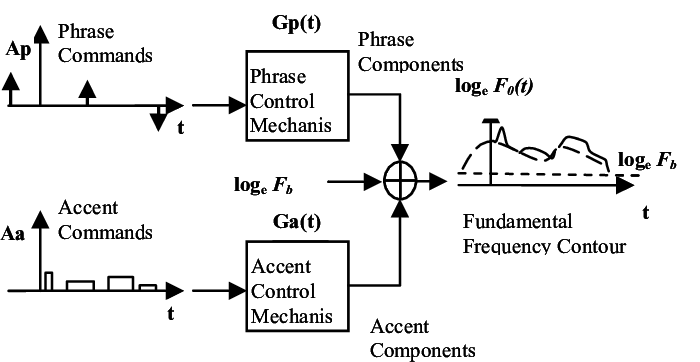
\includegraphics[scale=1.2]{figures/fujisaki-model.png}
\caption[The Fujisaki model]{The Fujisaki Model. Reprinted from \citet{Fujisaki2002modeling}.}
\end{figure}


Phrase commands and accent commands are said to simulate the action of laryngeal muscles that control the frequency of vibration of the vocal cords. 
This endows the model with a strong physiological basis.

As the placement of phrase commands and accent commands often corresponds to key phonological units such as accent groups and phrase boundaries, the model is able to produce linguistically interpretable commands.



\subsection{The IPO Model}

Initially introduced to model Dutch intonation, the IPO model of intonation \citep{Gussenhoven1992Perceptual} is generally classified as a perception-based model of intonation.
This is because this approach relies on a number of assumptions about how contours are perceived by humans.

In particular, the IPO model puts forward that \ac{F0} changes that cannot be perceived by humans need not be modeled and that it is sufficient to only model perceptually salient features of pitch.
Additionally, the IPO approach is based on the assumption that the human ear is more sensitive to tone variations (i.e., rise versus fall), than tone intensities (i.e., high versus low).

Because on these assumptions, the IPO approach does not model raw \ac{F0} contours, but rather piece-wise linear approximations superimposed on a general declination line that are perceptually indistinguishable from the original, as shown in \autoref{fig:ipo-stylization}.


\begin{figure}[H]
\centering
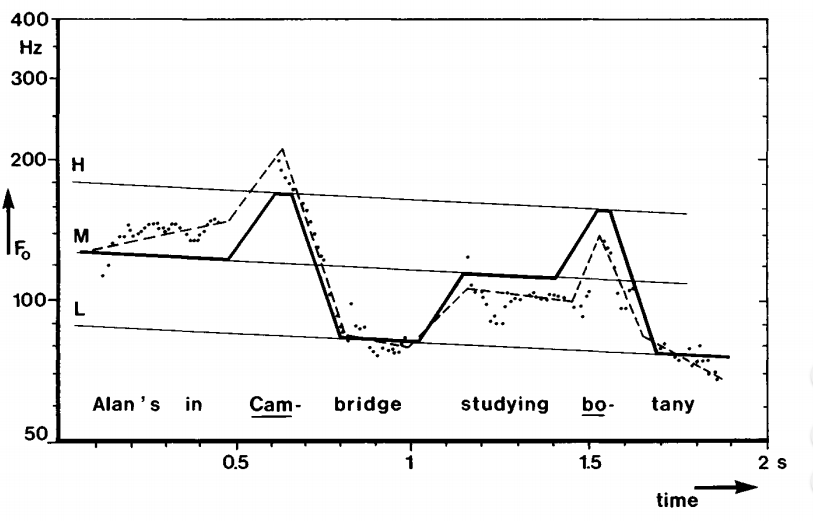
\includegraphics[scale=0.5]{figures/ipo-contour-stylization.png}
\caption[IPO model contour approximation]{Example of a piece-wise linear approximation of a contour. Reprinted from \citet[p.\ 49]{Gussenhoven1992Perceptual}.}
\label{fig:ipo-stylization}
\end{figure}

After these approximations are produced, contours can be broken down into a fixed inventory of \ac{F0} movements that are capable of describing the whole original speech corpus from which they were extracted.
The combinations of these \ac{F0} movements are described by a grammar.


\subsection{The Tilt Model}

The tilt intonation model was first introduced by \citet{Taylor1994Rise} and is based on his \emph{rise/fall/connection} model of intonation.
As this model is based on a shape-based description of prosodic events, it has been classified as an acoustic stylization-based model.

The model is based on four building blocks: pitch accents (modeled by combinations of quadratic functions), boundary tones (also modeled by combinations of quadratic functions), connections (modeled by straight-line interpolations) and silences.

These building blocks can be used to describe prosodic events.
In the model, each event is a associated with a set of parameters.
Each set of parameters includes the position of the intonational event within both the time and frequency domains, the amplitude, the duration, as well as a so-called \emph{tilt} value.

A tilt value is a real-valued parameter that describes the shape of the event and is calculated by dividing the difference of the rise and fall of the amplitudes of the quadratic functions by their sum:

\begin{equation}
tilt = \dfrac{|A_{rise}| - |A_{fall}|}{|A_{rise}| + |A_{fall}|}
\label{frequency-equation}
\end{equation}
where:
\begin{conditions}
A_{rise}    &  amplitude of the rise \\
A_{rise}  &  amplitude of the fall
\end{conditions}

The tilt parameters can range between $-1$ and $1$, where $-1$ represents a pure fall, $0$ a perfectly symmetrical peak, and $1$ a pure rise.

% the acro thing messes up the title
\subsection{HMM and DNN Approaches}

Over the past couple of decades, there have been a number of attempts of modeling the \ac{F0} by means of \acp{HMM} and \acp{DNN}.
Multiple \ac{F0} prediction models have been developed for the \ac{HMM} paradigm \citep{Latorre2008Multilevel, Yu2009Probablistic, Yu2011Continuous}.
However, as \acp{DNN} have been shown to outperform \acp{HMM}, various flavors and combinations of neural network architectures for the modeling of the \ac{F0} have been proposed, from \acp{FFNN} \citep{Vainio2001Artificial}, to \acp{RNN} \citep{Zen2015Unidirectional}, to \acp{BRNN} \citep{Fan2014TTS}, etc.

Aside from the type of architecture, neural network approaches can be classified based on whether prosody is modeled by a dedicated model \citep[e.g.,][]{Vainio2001Artificial, Traber1990F0} or jointly with other speech features \citep[e.g.,][]{Zen2015Unidirectional, Fan2014TTS}.
The latter approach has become more common in the last few years and is consistent with the more general trend in \ac{TTS} technology towards increasingly end-to-end systems.
This is also the approach found in the open-source Merlin toolkit for \ac{DNN} synthesis \citep{Wu2016Merlin}.

The main idea behind this trend is to minimize human effort and intervention in the task of feature engineering as much as possible.
In spite of its convenience, this approach is also less modular and less flexible, especially for the purpose of research.

\acp{DNN} are notoriously hard to examine, because they produce highly distributed representations, where it is not easy to determine for which aspects each parameter is responsible.
When \ac{DNN} \ac{F0} modeling is performed jointly with other speech features, the \ac{F0} contour is intrinsically tied to the other features.
This means that if we try to replace the \ac{F0} contour with a different one, the other features will not change to suite the new contour.

Another aspect by which neural network approaches may differ is how much (or how little) the \ac{F0} contour is pre-processed.
One extreme case is when \ac{F0} contours are only minimally processed by means of a simple log transform.
Aside from this extreme, there are a number of approaches with various levels of pre-processing such as Fujisaki model inspired approaches \citep{Sakurai2000Data}, \ac{F0} template approaches \citep{Ronanki2016Template}, quantization approaches \citep{Wang2017RNN}, \ac{DCT} approaches \citep{Yin2016Modeling}, etc. 

Among the previous work focusing on intonation modeling in \ac{SPSS}, where significant processing is carried out, the most recent studies concern the use of wavelets \citep{Suni2013Wavelets, Vainio2013Continuous, Ribeiro2015Multi, Ribeiro2016Wavelet}.
In particular, the \ac{CWT} has proven useful both for analysis \citep{Vainio2013Continuous}, as well as modeling \citep{Suni2013Wavelets}.
Further, it has been shown that \ac{CWT} can be used to decompose the \ac{F0} contour into various components based on different prosodic scales (phrase, word, syllable, etc.), where not all components are equally relevant for the reconstructed signal \citep{Ribeiro2015Multi}.
Low frequencies do not convey much prosodic information, and high frequencies are mostly noise.
Wavelet contours can be stylized for each prosodic level by means of \ac{DCT}.
This approach was successfully applied also in the context of \ac{DNN} synthesis, and it was shown to produce more natural sounding prosody  \citep{Ribeiro2016Wavelet}.



\section{Proposed Methodology}

In this section, I outline a deep learning methodology for the modeling of intonation in the context of \ac{SPSS}.
The advantages of \ac{SPSS} have been amply explored in \autoref{sec:tts-paradigms}, including the freedom to model the \ac{F0} independently of other speech features.
In the proposed methodology, the \ac{F0} is generated by a dedicated \ac{DNN} model, while other acoustic features are generated by a separate \ac{DNN} model implemented for the synthesis of segmental features.

In \autoref{sec:intonation-models}, I presented the historically most influential theories, models and approaches for the modeling of intonation.
One common feature shared by most of the previous work is either a fully or partially static representation of intonation.
For instance, Pierrehumbert's theory of intonation is based on a binary contrast of static high and low tones, the Fujisaki model is based on the superimposition of functions that output static contour values, wavelets decompose contours into static hierarchically organized sub-components, etc.

The IPO and the Tilt models display a higher level of dynamism as contours are described in terms of fall and rise.
However, these approaches are not fully dynamic.
For instance, under the IPO approach, contours are synthesized from a fixed inventory of standardized pitch templates, where the position of the templates within the frequency domain is determined by the general declination line on which they are superimposed.

The Tilt model is more flexible than the IPO model, as the shape of prosodic events is not determined by a fixed inventory of pitch movements, but rather by a set of \emph{tilt} parameters.
The Tilt model is also somewhat dynamic, because each event is described in terms of fall/rise, instead of a static high/low opposition.
However, the start of each event is a static frequency value that anchors the fall/rise pattern within a specific region of the frequency domain.

In this thesis, I propose a purely dynamic approach, in which we model the dynamic evolution of the interpolated \ac{F0} through time from a starting position.
The dynamic information is parametrized by a sign value for the direction of change, and a quantized magnitude value for the amount of change in such direction.
The overall position of the predicted contour within the frequency domain is determined based on the speaker's voice register.

Unlike the Fujisaki model and wavelet approaches, in the proposed methodology, contours are not decomposed into hierarchical sub-components.
Similarly to the Tilt model, they are encoded into sequences of intonational events, where each event represents a pitch movement.
Unlike the Tilt model, the position of each event within the frequency domain is not static, but rather relative to the previous event.

Finally, the proposed methodology takes advantage of the recent advances in deep learning technology by also including word embeddings in the model, so that contour predictions are driven by semantically richer information.
